\section{Introduction}
\label{sec:introduction}

\subsection{Motivation}
\label{sec:motivation}

Most Linux distributions are either conservative remixes of existing systems or
highly opinionated tools for a specific niche. Neither describes this project.

The dominant desktop operating systems have a structural problem. Windows works
against its own users: forced updates, advertisements in the start menu, and
background telemetry that nobody enabled and cannot be fully disabled. The German
Federal Office for Information Security (BSI) has studied this directly: as part
of the SiSyPHuS research programme, the BSI found that required diagnostic data
collection in Windows~10 and~11 runs continuously and cannot be turned off by
the user~\cite{bsi2022sisyphus}. macOS presents a different trade-off: its
privacy posture is meaningfully better than Windows, but the ecosystem is
deliberately constructed to keep users paying and dependent. A 2024 study
published at CHI found that even opting out of Apple's analytics during device
setup does not prevent data collection by individual system applications, and
that the setup process itself involves at least eight distinct data-sharing
decisions presented in ways that are not straightforward to review~\cite{kollnig2024apple}.
Every Linux distribution, however technically sound, has failed to reach people
who simply want to use a computer without becoming a system administrator. The
gap between technically capable and actually usable has not closed in thirty years.

This project exists to close that gap. It is a Linux-based operating system
designed around a different set of priorities: one that integrates a
system-wide knowledge graph, AI interfaces, and modern tooling not as features
bolted on top, but as foundational infrastructure. It takes a clear stance on
user sovereignty, independence from dominant platform vendors, and not being
annoying to use.
If an operating system is being built in 2025 anyway, there is no reason to
repeat patterns from 1995.

\subsection{Target Audience}
\label{sec:audience}

The primary audience is people switching from macOS or Windows who want a
genuinely good alternative: modern in appearance, functional out of the box,
and respectful of their autonomy. Consumer-first, not enterprise-first. The
macOS user tired of lock-in but unwilling to compromise on quality. The Windows
user whose computer feels like it belongs to Microsoft more than to them. They
do not want to configure. They want to arrive and work, and feel like the
operating system is actually theirs.

Business deployment is a supported use case. The architecture accommodates
managed environments and administrator policies. The user remains the primary
stakeholder regardless of deployment context: an administrator can configure
defaults and restrict software; an administrator cannot surveil users or
override their personal data ownership. The system is not enterprise-first;
it is user-first by design, in every context.

\subsection{Design Principles}
\label{sec:principles}

The following principles govern every design decision in this project. They are
not aspirational language; they are constraints that break ties and override
convenience.

The user's interests come first. No advertisements, no tracking, no dark patterns,
no telemetry without explicit consent. This applies in managed environments too:
an organization can configure and restrict, but cannot surveil. All system
intelligence runs locally. The knowledge graph, AI context, and activity history
do not leave the machine without an explicit user action. The system works fully
offline, without registration, and without depending on services controlled by
companies in other jurisdictions. Cloud features are opt-in extensions, not
prerequisites. This is a technical commitment. It means the architecture enforces
it, not just the privacy policy.

The system has to be genuinely good to use. Everything works on first boot. No
hunting for drivers, no reading wiki pages to get audio working. The interface
must look better than what users are coming from, because a poor interface is a
barrier to entry regardless of what is underneath it. Small things matter more
than large ones: a system that remembers what you were working on, or switches
themes everywhere in one action, earns trust faster than an impressive feature
nobody uses. Coherence matters too: shared configuration, shared theming, shared
interfaces across all components. No part of the system should look like it was
designed in a different decade by a different team.

New technology gets used when it makes sense, not because it is trending. AI
and the knowledge graph are here because they genuinely change what a personal
computer can do for the user. The goal is a useful, trustworthy system, not a
clean architecture. Where established standards exist, this project builds
compatibility bridges rather than replacements. Apps built for other Linux
desktops run here; standard hardware interfaces work; nothing is deliberately
broken for the sake of purity. The system can explain what it is doing, in
plain language, in a place the user can see and act on it.

\subsection{Positioning}
\label{sec:positioning}

Figure~\ref{fig:positioning} maps the design space along two axes: how easy
the system is to use for a non-technical user, and how much sovereignty the
user has over their own data and software environment. These two properties
have historically traded off against each other. Mainstream commercial systems
prioritize usability but compromise on sovereignty, typically through telemetry,
ecosystem lock-in, or both. The more privacy-conscious Linux distributions give
users genuine control but impose a real usability cost. The upper-right
quadrant, high usability \emph{and} high user sovereignty, is where this
project aims to land. No system targeting mainstream usability currently occupies it.

\begin{figure}[htbp]
\centering
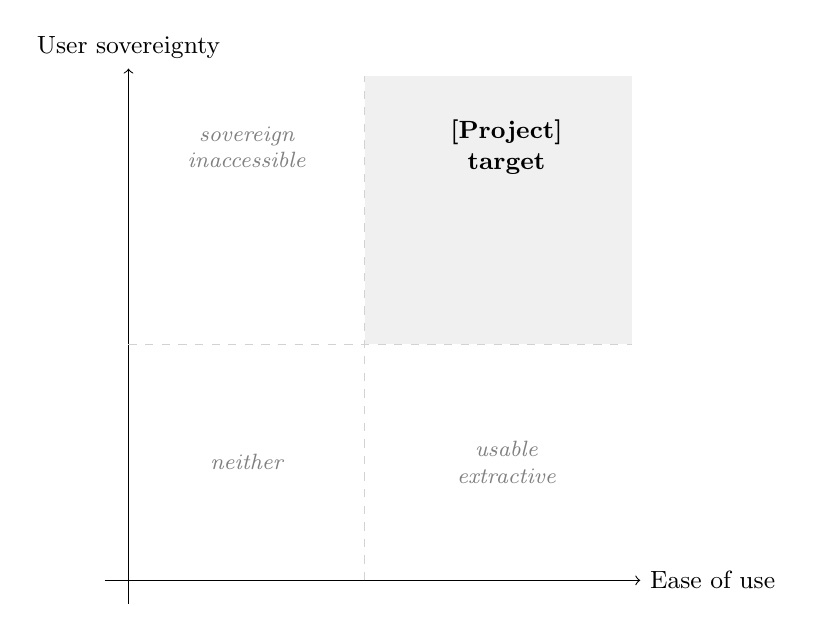
\begin{tikzpicture}
  % Axes
  \draw[->] (-0.3,0) -- (6.5,0)
    node[right, font=\small] {Ease of use};
  \draw[->] (0,-0.3) -- (0,6.5)
    node[above, font=\small] {User sovereignty};

  % Quadrant dividers
  \draw[gray!35, dashed] (3,0) -- (3,6.4);
  \draw[gray!35, dashed] (0,3) -- (6.4,3);

  % Target quadrant highlight
  \fill[gray!12] (3,3) rectangle (6.4,6.4);

  % Quadrant labels
  \node[gray, font=\footnotesize\itshape, align=center]
    at (1.5, 5.5) {sovereign\\inaccessible};
  \node[gray, font=\footnotesize\itshape, align=center]
    at (4.8, 1.5) {usable\\extractive};
  \node[gray, font=\footnotesize\itshape, align=center]
    at (1.5, 1.5) {neither};

  % Project target
  \node[font=\small\bfseries, align=center]
    at (4.8, 5.5) {[Project]\\target};

\end{tikzpicture}
\caption{Design space: ease of use versus user sovereignty. The shaded quadrant
is the project target. Mainstream commercial systems land in the lower-right
(usable but extractive); privacy-oriented Linux distributions in the upper-left
(sovereign but inaccessible). No mainstream system currently occupies the
upper-right.}
\label{fig:positioning}
\end{figure}

\subsection{What This Project Is Not}
\label{sec:nongoals}

Clarifying what this project is not is as important as describing what it is.

It is not a minimal system stripped to its essentials. There is real complexity
here, and that is intentional: a system that works for non-technical users
requires more infrastructure, not less.

It is not a fully declarative system where every piece of software is managed
through configuration files. Reproducibility is a goal; mandatory declarative
configuration is not.

It is not a distro aimed at advanced Linux users only. New users are explicitly
part of the target. Advanced users are welcome and well-served, but they are not
the primary design constraint.

It is not an enterprise product that happens to support consumers. The
design constraint is the non-technical user; business features exist where
they do not compromise that.

It is not a Windows or macOS clone. The goal is a better alternative, not a
familiar imitation.
